% version 1.2 dated 09 May 2011

% This file (c) 2009-2011 Elsevier Ltd.  Modifications may be freely made,
% provided the edited file is saved under a different name

% This file contains modifications for Procedia Computer Science

% Changes since version 1.1
% - added "procedia" option compliant with ecrc.sty version 1.2a
%   (makes the layout approximately the same as the Word CRC template)
% - added example for generating copyright line in abstract

%-----------------------------------------------------------------------------------

%% This template uses the elsarticle.cls document class and the extension package ecrc.sty
%% For full documentation on usage of elsarticle.cls, consult the documentation "elsdoc.pdf"
%% Further resources available at http://www.elsevier.com/latex

%-----------------------------------------------------------------------------------

%%%%%%%%%%%%%%%%%%%%%%%%%%%%%%%%%%%%%%%%%%%%%%%%%%%%%%%%%%%%%%
%%%%%%%%%%%%%%%%%%%%%%%%%%%%%%%%%%%%%%%%%%%%%%%%%%%%%%%%%%%%%%
%%                                                          %%
%% Important note on usage                                  %%
%% -----------------------                                  %%
%% This file should normally be compiled with PDFLaTeX      %%
%% Using standard LaTeX should work but may produce clashes %%
%%                                                          %%
%%%%%%%%%%%%%%%%%%%%%%%%%%%%%%%%%%%%%%%%%%%%%%%%%%%%%%%%%%%%%%
%%%%%%%%%%%%%%%%%%%%%%%%%%%%%%%%%%%%%%%%%%%%%%%%%%%%%%%%%%%%%%

%% The '3p' and 'times' class options of elsarticle are used for Elsevier CRC
%% The 'procedia' option causes ecrc to approximate to the Word template
\documentclass[3p,times,procedia]{elsarticle}
\flushbottom

%% The `ecrc' package must be called to make the CRC functionality available
\usepackage{ecrc}
%\usepackage{parskip}
\usepackage{amsmath}
\usepackage{ragged2e}
\usepackage{graphicx}
\usepackage{float}


%% The ecrc package defines commands needed for running heads and logos.
%% For running heads, you can set the journal name, the volume, the starting page and the authors

%% set the volume if you know. Otherwise `00'
%%\volume{}

%% set the starting page if not 1
\firstpage{1}

%% Give the name of the journal
\journalname{Computational Intelligence, Spring 2022}

%% Give the author list to appear in the running head
%% Example \runauth{C.V. Radhakrishnan et al.}
\runauth{}

%% The choice of journal logo is determined by the \jid and \jnltitlelogo commands.
%% A user-supplied logo with the name <\jid>logo.pdf will be inserted if present.
%% e.g. if \jid{yspmi} the system will look for a file yspmilogo.pdf
%% Otherwise the content of \jnltitlelogo will be set between horizontal lines as a default logo

%% Give the abbreviation of the Journal.
%% \jid{}

%% Give a short journal name for the dummy logo (if needed)
%\jnltitlelogo{Computer Science}

%% Hereafter the template follows `elsarticle'.
%% For more details see the existing template files elsarticle-template-harv.tex and elsarticle-template-num.tex.

%% Elsevier CRC generally uses a numbered reference style
%% For this, the conventions of elsarticle-template-num.tex should be followed (included below)
%% If using BibTeX, use the style file elsarticle-num.bst

%% End of ecrc-specific commands
%%%%%%%%%%%%%%%%%%%%%%%%%%%%%%%%%%%%%%%%%%%%%%%%%%%%%%%%%%%%%%%%%%%%%%%%%%

%% The amssymb package provides various useful mathematical symbols

\usepackage{amssymb}
%% The amsthm package provides extended theorem environments
%% \usepackage{amsthm}

%% The lineno packages adds line numbers. Start line numbering with
%% \begin{linenumbers}, end it with \end{linenumbers}. Or switch it on
%% for the whole article with \linenumbers after \end{frontmatter}.
%% \usepackage{lineno}

%% natbib.sty is loaded by default. However, natbib options can be
%% provided with \biboptions{...} command. Following options are
%% valid:

%%   round  -  round parentheses are used (default)
%%   square -  square brackets are used   [option]
%%   curly  -  curly braces are used      {option}
%%   angle  -  angle brackets are used    <option>
%%   semicolon  -  multiple citations separated by semi-colon
%%   colon  - same as semicolon, an earlier confusion
%%   comma  -  separated by comma
%%   numbers-  selects numerical citations
%%   super  -  numerical citations as superscripts
%%   sort   -  sorts multiple citations according to order in ref. list
%%   sort&compress   -  like sort, but also compresses numerical citations
%%   compress - compresses without sorting
%%
%% \biboptions{authoryear}

% \biboptions{}

% if you have landscape tables
\usepackage[figuresright]{rotating}
%\usepackage{harvard}
% put your own definitions here:x
%   \newcommand{\cZ}{\cal{Z}}
%   \newtheorem{def}{Definition}[section]
%   ...

% add words to TeX's hyphenation exception list
%\hyphenation{author another created financial paper re-commend-ed Post-Script}

% declarations for front matter


\begin{document}
\begin{frontmatter}

%% Title, authors and addresses

%% use the tnoteref command within \title for footnotes;
%% use the tnotetext command for the associated footnote;
%% use the fnref command within \author or \address for footnotes;
%% use the fntext command for the associated footnote;
%% use the corref command within \author for corresponding author footnotes;
%% use the cortext command for the associated footnote;
%% use the ead command for the email address,
%% and the form \ead[url] for the home page:
%%
%% \title{Title\tnoteref{label1}}
%% \tnotetext[label1]{}
%% \author{Name\corref{cor1}\fnref{label2}}
%% \ead{email address}
%% \ead[url]{home page}
%% \fntext[label2]{}
%% \cortext[cor1]{}
%% \address{Address\fnref{label3}}
%% \fntext[label3]{}

%\dochead{Middle East Technical University, Spring 2023}%

%% Use \dochead if there is an article header, e.g. \dochead{Short communication}
%% \dochead can also be used to include a conference title, if directed by the editors
%% e.g. \dochead{17th International Conference on Dynamical Processes in Excited States of Solids}

\title{\textbf{Training Artificial Neural Networks}}

%% use optional labels to link authors explicitly to addresses:
%% \author[label1,label2]{<author name>}
%% \address[label1]{<address>}
%% \address[label2]{<address>}



\author[]{Ozgur Gulsuna} 
%\author[b]{Second Author}
%\author[a,b]{Third Author\corref{cor1}}

\address[]{Middle East Technical University, Electrical and Electronics Engineering, Ankara, Turkey}
%\address[b]{Second affiliation, Address, City and Postcode, Country}

\begin{abstract}
%% Text of abstract
Insert here your abstract text.
\end{abstract}

\begin{keyword}
Type your keywords here, separated by semicolons ; 

%% keywords here, in the form: keyword \sep keyword

%% PACS codes here, in the form: \PACS code \sep code

%% MSC codes here, in the form: \MSC code \sep code
%% or \MSC[2008] code \sep code (2000 is the default)
\end{keyword}
%\cortext[cor1]{Corresponding author. Tel.: +0-000-000-0000 ; fax: +0-000-000-0000.}
\end{frontmatter}

%\correspondingauthor[*]{Corresponding author. Tel.: +0-000-000-0000 ; fax: +0-000-000-0000.}
\email{ozgur.gulsuna@metu.edu.tr}

%%
%% Start line numbering here if you want
%%
% \linenumbers

%% main text

\enlargethispage{10mm}
\section{\textbf{Basic Concepts}}
\label{main}

Here introduce the paper, and put a nomenclature if necessary, in a box with the same font size as the rest of the paper. The paragraphs continue from here and are only separated by headings, subheadings, images and formulae. The section headings are arranged by numbers, bold and 10 pt. Here follows further instructions for authors.

% \begin{nomenclature}
% \begin{deflist}[A]
% \defitem{A}\defterm{radius of}
% \defitem{B}\defterm{position of}
% \defitem{C}\defterm{further nomenclature continues down the page inside the text box}
% \end{deflist}
% \end{nomenclature}

\subsection{\textbf{Which Function ?}}

An ANNs classifier that is trained with cross-entropy loss approximates the conditional probability distribution function.
More specifically, for an input data, the output of the classifier is a probability distribution for the classes.
The cross-entorpy loss function is a measure between the predicted probability distribution and the true distribution.
The form of the loss function is decreasing, smooth and differentiable, which makes it easier to optimize using gradient-based methods.
This form is also known as the negative log-like function.

% An ANNs classifier trained with cross-entropy loss approximates a conditional probability distribution. Specifically, given an input vector, the classifier outputs a probability distribution over the possible classes that the input could belong to. The cross-entropy loss is defined as the negative log-likelihood of the correct class given the input.
% The reason why cross-entropy loss is used to approximate this function is that it is well-suited for optimizing models that output probability distributions. The loss encourages the model to assign a high probability to the correct class and low probabilities to the incorrect classes, which is exactly what we want from a classifier. The negative log-likelihood also has desirable properties such as being continuous and differentiable, making it easier to optimize using gradient-based methods.

% Bulleted lists may be included and should look like this:
% \begin{itemize}[]
% \item First point
% \item Second point
% \item And so on
% \end{itemize}

\subsection{\textbf{Gradient Computation}}
\subsection{\textbf{Some Training Parameters and Basic Parameter Calculations}}
\begin{enumerate}
    \item The batch refers to a subset of the training data that is used to compute the weights for one iteration. More specifically, the batch size is the number of training samples in a batch.
 The epoch on the other hand refers to the number of times the entire training data is used to update the weights. In training, there are generally multiple epoch iterations where the weights are updated with different batches/subsets of the training data.
    \item For the $N$ number of training samples, the number of batches per epoch is $N/B$, where $B$ is the batch size. A little side note that the solution is rounded up to the higher integer if $N/B$ is not an integer.
    \item For the optimization iterations, such as SGD, for $E$ number of epochs, the total number of iterations is $E \times N/B$. Again, a practical side note states that the $N/B$ is rounded up to the higher integer.
\end{enumerate}
\subsection{\textbf{Computing Number of Parameters of ANN Classifiers}}
\begin{enumerate}
    \item Starting from the initial layer of the MLP, we have $D_{in}$ number of input neurons and $H_1$ number of neurons in first hidden layer. Also there are biases associated with 
each neuron. Therefore, the number of parameters of the each layer is,
    \vspace{-0.5cm}
    \begin{equation*}
    \begin{array}{r}
    \textrm{Input Layer} = D_{in} \times H_{1} \ +\ H_{1} \\
    \textrm{Hidden Layers}= H_1 \times H_2 + H_2\\
    \cdot \cdot \cdot \hspace{2em} \\
    \textrm{More Hidden Layers} = H_{k-1} \times H_k + H_k\\
    \textrm{Output Layer} = H_{k} \times D_{out} \ +\ D_{out} \\
    \end{array}
    \end{equation*}

    \vspace{-0.25cm}
    The total sum can be written as, where $K$ is the number of hidden layers.
    \vspace{-0.5cm}
    \begin{equation*}
        \textrm{Total Number of Parameters} = D_{in}\times H_1 + \sum_{k=2}^{K} (H_{k-1} \times H_k + H_k) + H_k \times D_{out} +  D_{out}
    \end{equation*}
    \vspace{-0.25cm}

    \item CNN structure is more complicated. The number of parameters of a CNN layer is calculated as follows:
    
    For the input layer, the number of parameters is,
    \vspace{-0.5cm}
    \begin{equation*}
        \textrm{Input Layer} = (H_{in} \times W_{in} \times C_{in} \times C_1 )+ C_1
    \end{equation*}

    \vspace{-0.25cm}
    where $H_{in}$ and $W_{in}$ are the height and width of the input image, and $C_{in}$ is the number of channels of the input image.
    Each input of layer is the output of the previous layer.
    For the convolutional layers, the number of parameters is calculated as,
    \vspace{-0.5cm}
    \begin{equation*}
        \begin{array}{c}
            \displaystyle \textrm{Convolutional Layer} = H_k \times W_k \times C_{k-1} \times C_k + C_k \\
            \\
            \displaystyle \textrm{Combination of all layers is,} \\
            \displaystyle \textrm{Convolutional Layers} = \sum_{k=2}^{K} H_k \times W_k \times C_{k-1} \times C_k + C_k \\ 
        \end{array}
    \end{equation*}

    \vspace{-0.25cm}
    Here all the parameters are summed up. The output is assumed to be the last index of the array.
    The final equation for the total number of parameters is,
    \vspace{-0.5cm}
    \begin{equation*}
        \textrm{Total Number of Parameters} = (H_{in} \times W_{in} \times C_{in} \times C_1 )+ C_1 + \sum_{k=1}^{K} H_k \times W_k \times C_{k-1} \times C_k + C_k
    \end{equation*}

    \vspace{-0.25cm}

\end{enumerate}

% All tables should be numbered with Arabic numerals. Every table should have a caption. Headings should be placed above tables, left justified. Only horizontal lines should be used within a table, to distinguish the column headings from the body of the table, and immediately above and below the table. Tables must be embedded into the text and not supplied separately. Below is an example which the authors may find useful.

% \begin{table}[h]
% \caption{ An example of a table.}
% \begin{tabular*}{\hsize}{@{\extracolsep{\fill}}lll@{}}
% \toprule
% An example of a column heading & Column A ({\it{t}}) & Column B ({\it{t}})\\
% \colrule
% And an entry &   1 &  2\\
% And another entry  & 3 &  4\\
% And another entry &  5 &  6\\
% \botrule
% \end{tabular*}
% \end{table}

% %\enlargethispage{12pt}

\section{\textbf{Implementing a Convolutional Layer with NumPy}}

The section involves implementing conv2d function using NumPy for forward propagation and testing it on a small batch of MNIST dataset.
We downloaded and loaded input and kernel files, and created an output image using the part2Plots function.
The implementation code can be found in the appendix named my\_conv2d.py.
We confirmed the correctness of our implementation by the output image.
% References must be listed at the end of the paper. Do not begin them on a new page unless this is absolutely necessary. Authors should ensure that every reference in the text appears in the list of references and vice versa. Indicate references by \cite{Massimo2011} or \cite{Massimo2012} or \cite{Thomas2015} in the text.
% Some examples of how your references should be listed are given at the end of this template in the `References' section, which will allow you to assemble your reference list according to the correct format and font size.

% Reference generation by using bibliography style commands for LaTeX template only.

% The author may use ``elsarticle-harv.bst'' as per the style required in document. The sample bib file could be referred. 
% If the author may using bibstyle for providing references author must comment the bibliography section in TeX file, Bibtex will generate the reference automatically.

% If the author may not able to view the references in output same could be done by copying the bibliography section from ``filename.bbl'' file and paste in TeX file.



\subsection{\textbf{Experimental Work}}
The generated output for the convolution over the MNIST dataset is shown in Figure \ref{fig:output}.



\begin{figure}[H]
    \centering
    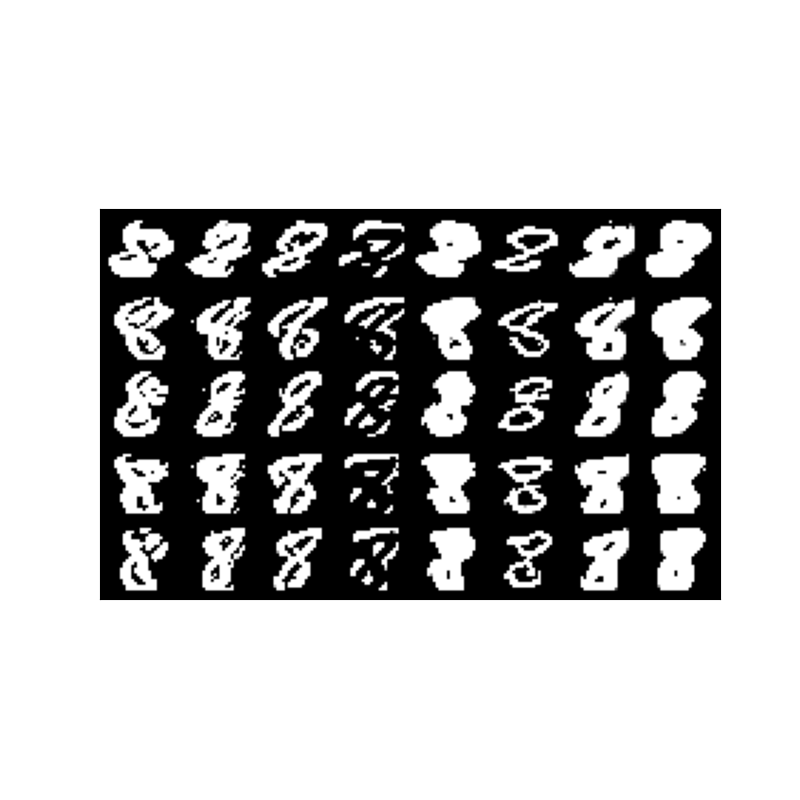
\includegraphics[width=0.5\textwidth, trim={0 5cm 0 5cm}]{figures/output.png}
    \caption{Convolution over the number 8 of the MNIST dataset}
    \label{fig:output}
\end{figure}

\vspace{-0.5cm}
\subsection{\textbf{Results and Discussion}}
\begin{enumerate}
    \item The Convolutional Neural Networks are important for couple of reasons.
    First of all, when the input shape of the CNN is selected as 2D, it is well suited image processing.
    Second, the CNN is able to learn the spatial features of the input image. This also means that the CNN is able to learn and extract the features of the input image without any manual work.
    CNN's are also able to recognize the features of the input image even if the input image is rotated or scaled.
    Since the features are extracted from image, partial occlusion of the image affect the performance of the CNN less.
    \item The kernel of a Convolutional Layer  is essentially a matrix of weights that is convolved (inversely correlated) over with the input data to extract features.
    The size of the kernel refers to the number of rows and columns in the matrix. It corresponds to the reception of the filter, meaning that higher sizes can extract more complex features. 
    
    \item The output image shows that the convolution of pre-presented kernels for the number 8 of the MNIST dataset. Basically each filter is convoled over the images to grasp different meanings. Each column is another kernel with each row is different input image.
    
    \item The numbers in the same column look like each other since they both have a representation of the same number and the same kernel is able to extract the features related to the number 8 other than the specific image.
    
    \item The numbers in the same row look different althougn the input image the same. This is because the kernels are different and they are able to extract different features from the same image.
    
    \item For more specific examples, the third column kernel represents that an 8 has two "islands" of white patches in the middle but the size, shape and location of these pathes differ for each 8 altough all of them represent the same thing in a different manner.
     Another column such as 6, implies the white track like feature of the number 8. In this sense some features are more dinstinctive than other however when different of these combined make the action work even though they do not seem to represent a clear feature.
     This is similar to human behaviour as we associate the similar patterns to the general inputs and this is the importance of the convolutaional layers, the features can be learned in a sense.
\end{enumerate}

\subsection{General guidelines for the preparation of your text}
Avoid hyphenation at the end of a line. Symbols denoting vectors and matrices should be indicated in bold type. Scalar variable names should normally be expressed using italics. Weights and measures should be expressed in SI units. All non-standard abbreviations or symbols must be defined when first mentioned, or a glossary provided.

\subsection{File naming and delivery}
Please title your files in this order `procedia acronym\_conference acronym\_authorslastname'.  Submit both the source file and the PDF to the Guest Editor.

Artwork filenames should comply with the syntax ``aabbbbbb.ccc'', where:
\begin{itemize}
\item a = artwork component type
\item b = manuscript reference code
\item c = standard file extension

Component types:
\item gr = figure
\item pl = plate
\item sc = scheme
\item fx = fixed graphic
\end{itemize}


\subsection{Footnotes}
Footnotes should be avoided if possible. Necessary footnotes should be denoted in the text by consecutive superscript letters\footnote{Footnote text.}. The footnotes should be typed single spaced, and in smaller type size (8 pt), at the foot of the page in which they are mentioned, and separated from the main text by a one line space extending at the foot of the column. The `Els-footnote' style is available in the ``TeX Template'' for the text of the footnote.

Please do not change the margins of the template as this can result in the footnote falling outside printing range.


\section{Illustrations}
All figures should be numbered with Arabic numerals (1,2,3,$\,\ldots.$). Every figure should have a caption. All\break photographs, schemas, graphs and diagrams are to be referred to as figures. Line drawings should be good\break quality scans or true electronic output. Low-quality scans are not acceptable. Figures must be embedded into the text and not supplied separately. In MS word input the figures must be properly coded. Preferred format of figures are PNG, JPEG, GIF etc. Lettering and symbols should be clearly defined either in the caption or in a legend provided as part of the figure. Figures should be placed at the top or bottom of a page wherever possible, as close as possible to the first reference to them in the paper. Please ensure that all the figures are of 300 DPI resolutions as this will facilitate good output.

The figure number and caption should be typed below the illustration in 8 pt and left justified [{\bfseries\itshape Note:} one-line captions of length less than column width (or full typesetting width or oblong) centered]. For more guidelines and\break information to help you submit high quality artwork please visit: http://www.elsevier.com/artworkinstructions\break Artwork has no text along the side of it in the main body of the text. However, if two images fit next to each other, these may be placed next to each other to save space. For example, see Fig.~1.
\begin{figure}[t]\vspace*{4pt}
%\centerline{\includegraphics{fx1}\hspace*{5mm}\includegraphics{fx1}}
%\centerline{\includegraphics{gr1}}
\caption{(a) first picture; (b) second picture.}
\end{figure}


\section{Equations}
Equations and formulae should be typed in MathType, and numbered consecutively with Arabic numerals in parentheses on the right hand side of the page (if referred to explicitly in the text). They should also be separated from the surrounding text by one space
\begin{equation}
\begin{array}{lcl}
\displaystyle X_r &=& \displaystyle\dot{Q}^{''}_{rad}\left/\left(\dot{Q}^{''}_{rad} + \dot{Q}^{''}_{conv}\right)\right.\\[6pt]
\displaystyle \rho &=& \displaystyle\frac{\vec{E}}{J_c(T={\rm const.})\cdot\left(P\cdot\left(\displaystyle\frac{\vec{E}}{E_c}\right)^m+(1-P)\right)}
\end{array}
\end{equation}


\section{Online license transfer}
All authors are required to complete the Procedia exclusive license transfer agreement before the article can be published, which they can do online. This transfer agreement enables Elsevier to protect the copyrighted material for the authors, but does not relinquish the authors' proprietary rights. The copyright transfer covers the exclusive rights to reproduce and distribute the article, including reprints, photographic reproductions, microfilm or any other reproductions of similar nature and translations. Authors are responsible for obtaining from the copyright holder, the permission to reproduce any figures for which copyright exists.

\section*{Acknowledgements}

Acknowledgements and Reference heading should be left justified, bold, with the first letter capitalized but have no numbers. Text below continues as normal.

%% The Appendices part is started with the command \appendix;
%% appendix sections are then done as normal sections
%% \appendix

%% \section{}
%% \label{}

\appendix
\section{An example appendix}
Authors including an appendix section should do so before References section. Multiple appendices should all have headings in the style used above. They will automatically be ordered A, B, C etc.

\subsection{Example of a sub-heading within an appendix}
There is also the option to include a subheading within the Appendix if you wish.
%% References
%%
%% Following citation commands can be used in the body text:
%% Usage of \cite is as follows:
%%   \cite{key}         ==>>  [#]
%%   \cite[chap. 2]{key} ==>> [#, chap. 2]
%%

%The citation must be used in following style: \cite{article-minimal} \cite{article-full} \cite{article-crossref} \cite{whole-journal}.
%% References with BibTeX database:

%\bibliography{xampl}
%\bibliographystyle{elsarticle-harv}


%% Authors are advised to use a BibTeX database file for their reference list.
%% The provided style file elsarticle-num.bst formats references in the required Procedia style

%% For references without a BibTeX database:

 \begin{thebibliography}{}

%% \bibitem must have the following form:
%%   \bibitem{key}...
%%

\bibitem{Massimo2011}
{F}ilippini, Massimo, and Lester C. Hunt. (2011) ``Energy demand and
energy efficiency in the OECD countries: a stochastic demand frontier
approach." {\it Energy Journal} {\bf 32} (2): 59--80.
\bibitem{Massimo2012}
Filippini, Massimo, and Lester C. Hunt. (2012) ``US residential
energy demand and energy efficiency: A stochastic demand frontier
approach." {\it Energy Economics} {\bf 34} (5): 1484--1491.
\bibitem{Thomas2015} 
Weyman-Jones, Thomas, J\'{u}lia Mendon\c{c}a Boucinha, and Catarina
Feteira In\'{a}cio. (2015) ``Measuring electric energy efficiency in
Portuguese households: a tool for energy policy." {\it Management of Environmental Quality: An International Journal} {\bf 26} (3): 407--422.
\bibitem{} 
Saunders, Harry (2009) ``Theoretical Foundations of the Rebound Effect'', in Joanne Evans and Lester Hunt (eds) {\it International Handbook on the Economics of Energy}, Cheltenham, Edward Elgar
\bibitem{} 
Sorrell, Steve (2009) ``The Rebound Effect: definition and estimation'', in Joanne Evans and Lester Hunt (eds) {\it International Handbook on the Economics of Energy}, Cheltenham, Edward Elgar 
 \end{thebibliography}

\clearpage

%%%% This page is for instructions only, once the article is finalize please omit the below text before creating the final PDF
\normalMode

\section*{Instructions to Authors for LaTeX template:}

\section{ZIP mode for LaTeX template:}

The zip package is created as per the guide lines present on the URL http://www.elsevier.com/author-schemas/ preparing-crc-journal-articles-with-latex for creating the LaTeX zip file of Procedia LaTeX template.  The zip generally contains the following files:
\begin{Itemize}[]\leftskip-17.7pt\labelsep3.3pt
\item ecrc.sty
\item  elsarticle.cls
\item elsdoc.pdf
\item .bst file
\item Manuscript templates for use with these bibliographic styles
\item  Generic and journal specific logos, etc.
\end{Itemize}

The LaTeX package is the main LaTeX template. All LaTeX support files are required for LaTeX pdf generation from the LaTeX template package. 

{\bf Reference style .bst file used for collaboration support:} In the LaTeX template packages of all Procedia titles a new ``.bst'' file is used which supports collaborations downloaded from the path http://www.elsevier.com/author-schemas/the-elsarticle-latex-document-class

\section{Reference style used in Computer Science:}
\let\footnotesize\normalsize
\hspace*{-10pt}\begin{tabular*}{\hsize}{@{}ll@{}}
{\bf Title}&{\bf Reference style} \\[6pt]
PROCS  & 3 Vancouver Numbered
\end{tabular*}

\end{document}

%%
%% End of file `procs-template.tex'.
